\chapter{Ergebnisse und Vergleich}
\label{chap:results}

Dieses Kapitel zeigt die Ergebnisse und den Vergleich zwischen den gewöhnlichen state-of-the-art Klassifizierern und den untersuchten RNN-Architekturen. Dabei wird zunächst ein Vergleich zwischen den klassischen und anschließend zwischen den komplexen Klassifikatoren gezogen. Abschließend werden die klassischen Klassifikatoren den RNN-Architekturen gegenübergestellt und die Ergebnisse beschrieben.

\section{Vergleich der gewöhnlichen Klassifikatoren}
\label{sec:other-classifiers-comp}

Beim Vergleich der gewöhnlichen Klassifikatoren fällt zunächst auf, dass alle für ihre vergleichsweise simple Architektur bereits gute Ergebnisse erzielen. Im Vergleich zu bisherigen Untersuchungen zu erwarten, waren die Ergebnisse der kNN und SVM. kNN sind laut \cite{Kaufmann2013} für gewöhnlich in Vergleichen die Klassifikatoren mit der geringsten Klassifikationsgenauigkeit. Trotzdem erreichten kNN in dieser Forschungsarbeit eine ausreichende Genauigkeit in einer vergleichsweise geringen Zeit, was sie zu einem validen Referenzwert macht. SVM erzielten vermutlich aufgrund ihrer nativen Minimierung von strukturiertem Risiko und der darauf resultierenden geringeren Tendenz zum Overfitting die im Hinblick auf die Klassifikationsgenauigkeit besten Ergebnisse. Gleichzeitig benötigten sie allerdings die zwischen allen state-of-the-art Klassifizierern in dieser Arbeit mit Abstand längste Trainingsdauer. Die im Rahmen der Arbeit untersuchte MLP Architektur erzielte zwar in einer im Vergleich zu SVM kurzen Zeit vergleichbar präzise Ergebnisse, tat sich allerdings schwer, diese selbst mit erhöhter Parameterzahl zu übertreffen. Um die Klassifizierungsgenauigkeit der MLP weiter zu optimieren, könnten diesen weitere HL unter sorgsamer Berücksichtigung der Overfitting-Problematik hinzugefügt werden. Eine tiefere Architektur mit zusätzlichen \textit{Dropout}-Schichten zur Sicherstellung der Generalisierbarkeit könnte verbesserte Ergebnisse liefern. Ausreißer in diesem Vergleich ist der untersuchte DT. Dieser liefert mit einer Klassifikationsgenauigkeit von 87,13\% eine Präzision nur leicht unter der der SVM in einem Bruchteil der Zeit. Hierzu sei allerdings hinzuzufügen, dass SVM durch weitere Optimierung, wie in vorheriger Forschung bereits zu sehen war bessere Ergebnisse erreichen und somit die Lücke zwischen DT und SVM vergrößern könnten (\cite{Kaufmann2013}). 

    \begin{table}[h]
        \centering
        \begin{tabular}{| l | c | c |}
            \hline
            \textbf{Klass.} & \textbf{Acc., \%} & \textbf{Dur., Min.} \\
            \hline
            SVM & 87,94 & 07:10 \\ \hline
            DT & 87,13 & 00:15 \\ \hline
            MLP & 86,14 & 03:01 \\ \hline
            kNN & 82,92 & 02:34 \\
            \hline
        \end{tabular}
        \caption{Ergebnisse der Cross Validation in Hinblick auf Klassifikationsgenauigkeit und Dauer aller untersuchter gewöhnlicher Klassifizierer, unterteilt in den verwendeten Klassifizierer (Klass.), die Klassifizierungsgenauigkeit (Acc.) und die Trainingsdauer (Dur.)}
        \label{tab:other-classifiers-comp}
    \end{table}

\section{Vergleich der RNN-Architekturen}
\label{sec:rnn-comp}

Im Fall der untersuchten RNN-Architekturen lassen sich einige Beobachtungen aufstellen. Die prägnanteste Erkenntnis dieses Experiments stellt die Klassifiezierungsleistung der gewöhnlichen RNN auf dem Validierungsdatensatz dar. Trotz weitreichender Optimierung der Hyperparameter und der Verwendung von Techniken wie dem Gradient Clipping erzielten gewöhnliche RNN im Vergleich zu den anderen RNN-Architekturen signifikant schlechtere Ergebnisse. Ihre zuletzt erzielte Klassifikationsgenauigkeit von 82,95\% übertrifft nur marginal die Leistung des kNN-Algorithmus auf dem Datensatz. Dieses Ergebnis überrascht vor allem deshalb, weil gewöhnliche RNN in vorigen Untersuchungen auf sEMG-Datensätzen bereits gute Ergebnisse erzielten, auch wenn diese im Vergleich zu den LSTM und GRU Architekturen meist dennoch schlechter ausfielen (\cite{simao2019emg}). Da RNN in der Forschung bis jetzt noch nicht mit dem in dieser Arbeit erforschten Datensatz untersucht wurden, könnte eine mögliche Erklärung für dieses Auftreten die länge der Sequenzen sein. Da gewöhnliche RNN häufig unter der Problematik des VG leiden, die vor allem bei langen Sequenzen zu Fehlklassifikationen führen kann, könnte dieser Schritt die Klassifikationsgenauigkeit stark erhöhen. Eine VG-Problematik könnte anhand des vorliegenden Graphen an der stetigen Abflachung der Klassifikationsgenauigkeits-Kurve erkannt werden, da dies auf geringe Anpassung in den Gewichten der Neuronen und somit auf einen sehr kleinen Gradienten hindeuten könnte. Gleichzeitig lässt sich anhand von Abbildung \ref{gra:rnn-comp} dieser Trend der Abflachung bereits ab der ersten Epoche beobachten. Während die Kurven der LSTM und GRU zunächst konvex verlaufen, ist die Trajektorie der gewöhnlichen RNN konstant konkav. Ein weiteres Indiz für eine VG Problematik lässt sich mit Blick auf die Diskrepanz zwischen der Leistung der gewöhnlichen RNN und den LSTM und GRU Architekturen erkennen. Diese speziell zur Lösung der VG- und EG-Problematik entwickelten Architekturen liefern nahezu identische Ergebnisse und eine dabei wesentlich höhere Präzision. Da diese Architekturen gewöhnlicherweise keine Schwierigkeiten mit der VG oder EG Problematik haben, könnte dies ebenfalls auf einen VG im Fall der gewöhnlichen RNN deuten. Die unmittelbarste Methode auf eine VG Problematik in den gewöhnlichen RNN zu prüfen, wäre das Untersuchen der Gradienten während des Trainings des Netzwerks. Tendieren diese gegen 0, liegt VG in der Architektur vor. Allerdings konnte dies aufgrund von technischen Einschränkungen in der verwendeten Tensorflow API im Verlauf dieser Arbeit nicht durchgeführt werden.

Ebenfalls hervorzuheben ist der Vergleich zwischen LSTM und GRU. Zwar ist die letztendlich erzielte Klassifikationsgenauigkeit der Architekturen nahezu identisch, GRU erreichen diese allerdings, wie in Tabelle \ref{tab:rnn-comp} zu sehen, in einem Drittel der Trainingsdauer und sind somit erwartungsgemäß schneller als LSTM. Das ist, wie bereits im vorgehenden Kapitel zu der Architektur angesprochen, auf die geringere Parameterzahl zurückzuführen.
\begin{table}[h]
    \centering
    \begin{tabular}{| l | c | c |}
        \hline
        \textbf{Arch.} & \textbf{Acc., \%} & \textbf{Dur., Min.} \\
        \hline
        GRU & 98,11 & 18:02 \\ \hline
        LSTM & 98,11 & 58:28 \\ \hline
        RNN & 82,95 & 46:14 \\

        \hline
    \end{tabular}
    \caption{Ergebnisse der Cross Validation in Hinblick auf Klassifizierungsgenauigkeit und Dauer aller untersuchter RNN-Architekturen, unterteilt in die verwendete Architektur (Arch.), die Klassifizierungsgenauigkeit (Acc.) und die Trainingsdauer (Dur.)}
    \label{tab:rnn-comp}
\end{table}

Die untersuchte GRU Architektur beinhaltet bei nahezu identischer Struktur lediglich inetwa 250.000 trainierbare Parameter, während die LSTM Struktur 360.000 enthält. Gleichzeitig lässt sich anhand von Abbildung \ref{gra:rnn-comp} beobachten, dass LSTM bereits in früheren Epochen genauere Ergebnisse erzielen als GRU. Dieser Unterschied ist allerdings für den Vergleich nicht ausschalggebend, da die Asymptotisierung zu einem ähnlichen Zeitpunkt, in etwa nach Epoche 24, eintritt.

\begin{figure}[h]
    \centering
    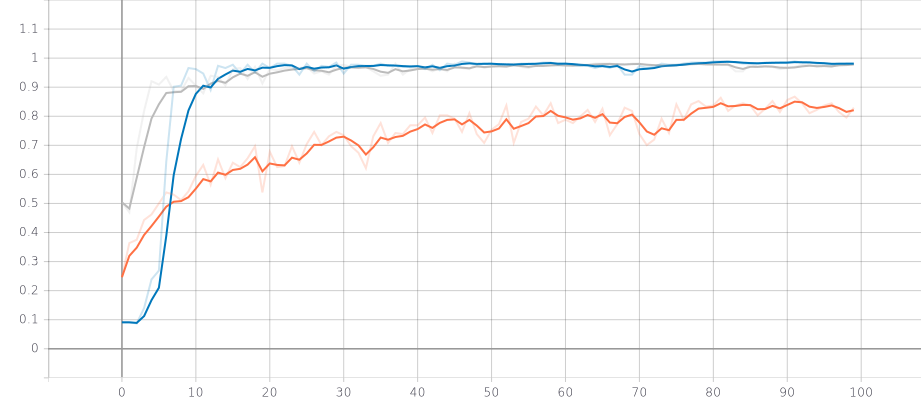
\includegraphics[scale=0.3]{grafiken/rnn-comp.png}
    \caption{Vergleich der Klassifizierungsgenauigkeiten in Abhängigkeit der Epoche. Enthalten sind das gewöhnliche RNN (Orange), LSTM (Grau) und GRU (Blau)}
    \label{gra:rnn-comp}
\end{figure}

Allgemein lässt sich somit sagen, dass nach den in dieser Forschungsarbeit untersuchten Kriterien die GRU Architektur mit einer Klassifikationsgenauigkeit von 89,11\% und einer Trainingsdauer von 18 Minuten und 2 Sekunden die besten Ergebnisse zwischen den RNN-Architekturen liefert.

\section{Vergleich zwischen gewöhnlichen Klassifikatoren und RNN}
\label{subsec:rnn-other-comp}

Betrachtet man nun abschließend alle untersuchten Klassifikatoren, so zeichnet sich sowohl in der Klassifikationsgenauigkeit als auch in der Trainingsdauer ein Unterschied ab. Während selbst der beste gewöhnliche Klassifizierer, die SVM, in etwa zehn Prozentpunkte schlechter in der Klassifikationsgenauigkeit abschneidet als die beste RNN Architektur, das GRU, so braucht dieser für das Ergebnis weniger als die Hälfte der Trainingsdauer. Ebenfalls zu beobachten ist im Vergleich zwischen den gewöhnlichen Klassifizierern und RNN-Architekturen die Tendenz zu besseren Klassifizierungsgenauigkeiten bei größerer Trainingsdauer. Diese allgemeine Tendenz macht sowohl GRU als auch DT besonders interessant, da diese den Trend brechen und trotz geringerer Trainingsdauer bessere Ergebnisse liefern als die mit ihnen direkt verglichenen Architekturen. Sowohl GRU, die als vergleichsweise junge Architektur noch am Anfang ihrer Optimierung stehen, als auch DT, deren Einsatz in Verbindung mit komplexeren Algorithmen auch im Rahmen der Klassifikation von EMG Signalen bereits gute Ergebnisse hervorbrachte (\cite{gokgoz2015comparison}), haben daher großes Potenzial für die Zukunft der Klassifikation von EMG Signalen.

\begin{table}[h]
    \centering
    \bgroup
    \begin{tabular}{| l | c | c |}
        \hline
        \textbf{Klass.} & \textbf{Acc., \%} & \textbf{Dur., Min.} \\
        \hline
        GRU & \textbf{98,11} & \textbf{18:02}\\ \hline
        LSTM & 98,11 & 58:28 \\ \hline
        RNN & 82,95 & 46:14 \\
        \hline
        \hline
        SVM & \textbf{87,94} & 07:10 \\ \hline
        DT & 87,13 & \textbf{00:15 }\\ \hline
        MLP & 86,14 & 03:01 \\ \hline
        kNN & 82,92 & 02:34 \\
        \hline
    \end{tabular}
    \egroup
    \caption{Ergebnisse der Cross Validation in Hinblick auf Klassifizierungsgenauigkeit und Dauer aller untersuchter Klassifikatoren, unterteilt in den verwendeten Klassifikator (Klass.), die Klassifizierungsgenauigkeit (Acc.) und die Trainingsdauer (Dur.)}
    \label{tab:rnn-comp}
\end{table}
